\documentclass[tikz,border=8pt]{standalone}
\usepackage{amsmath,amssymb}
\usetikzlibrary{arrows.meta,calc,decorations.markings,decorations.pathmorphing,patterns,shapes.geometric,positioning}

\begin{document}
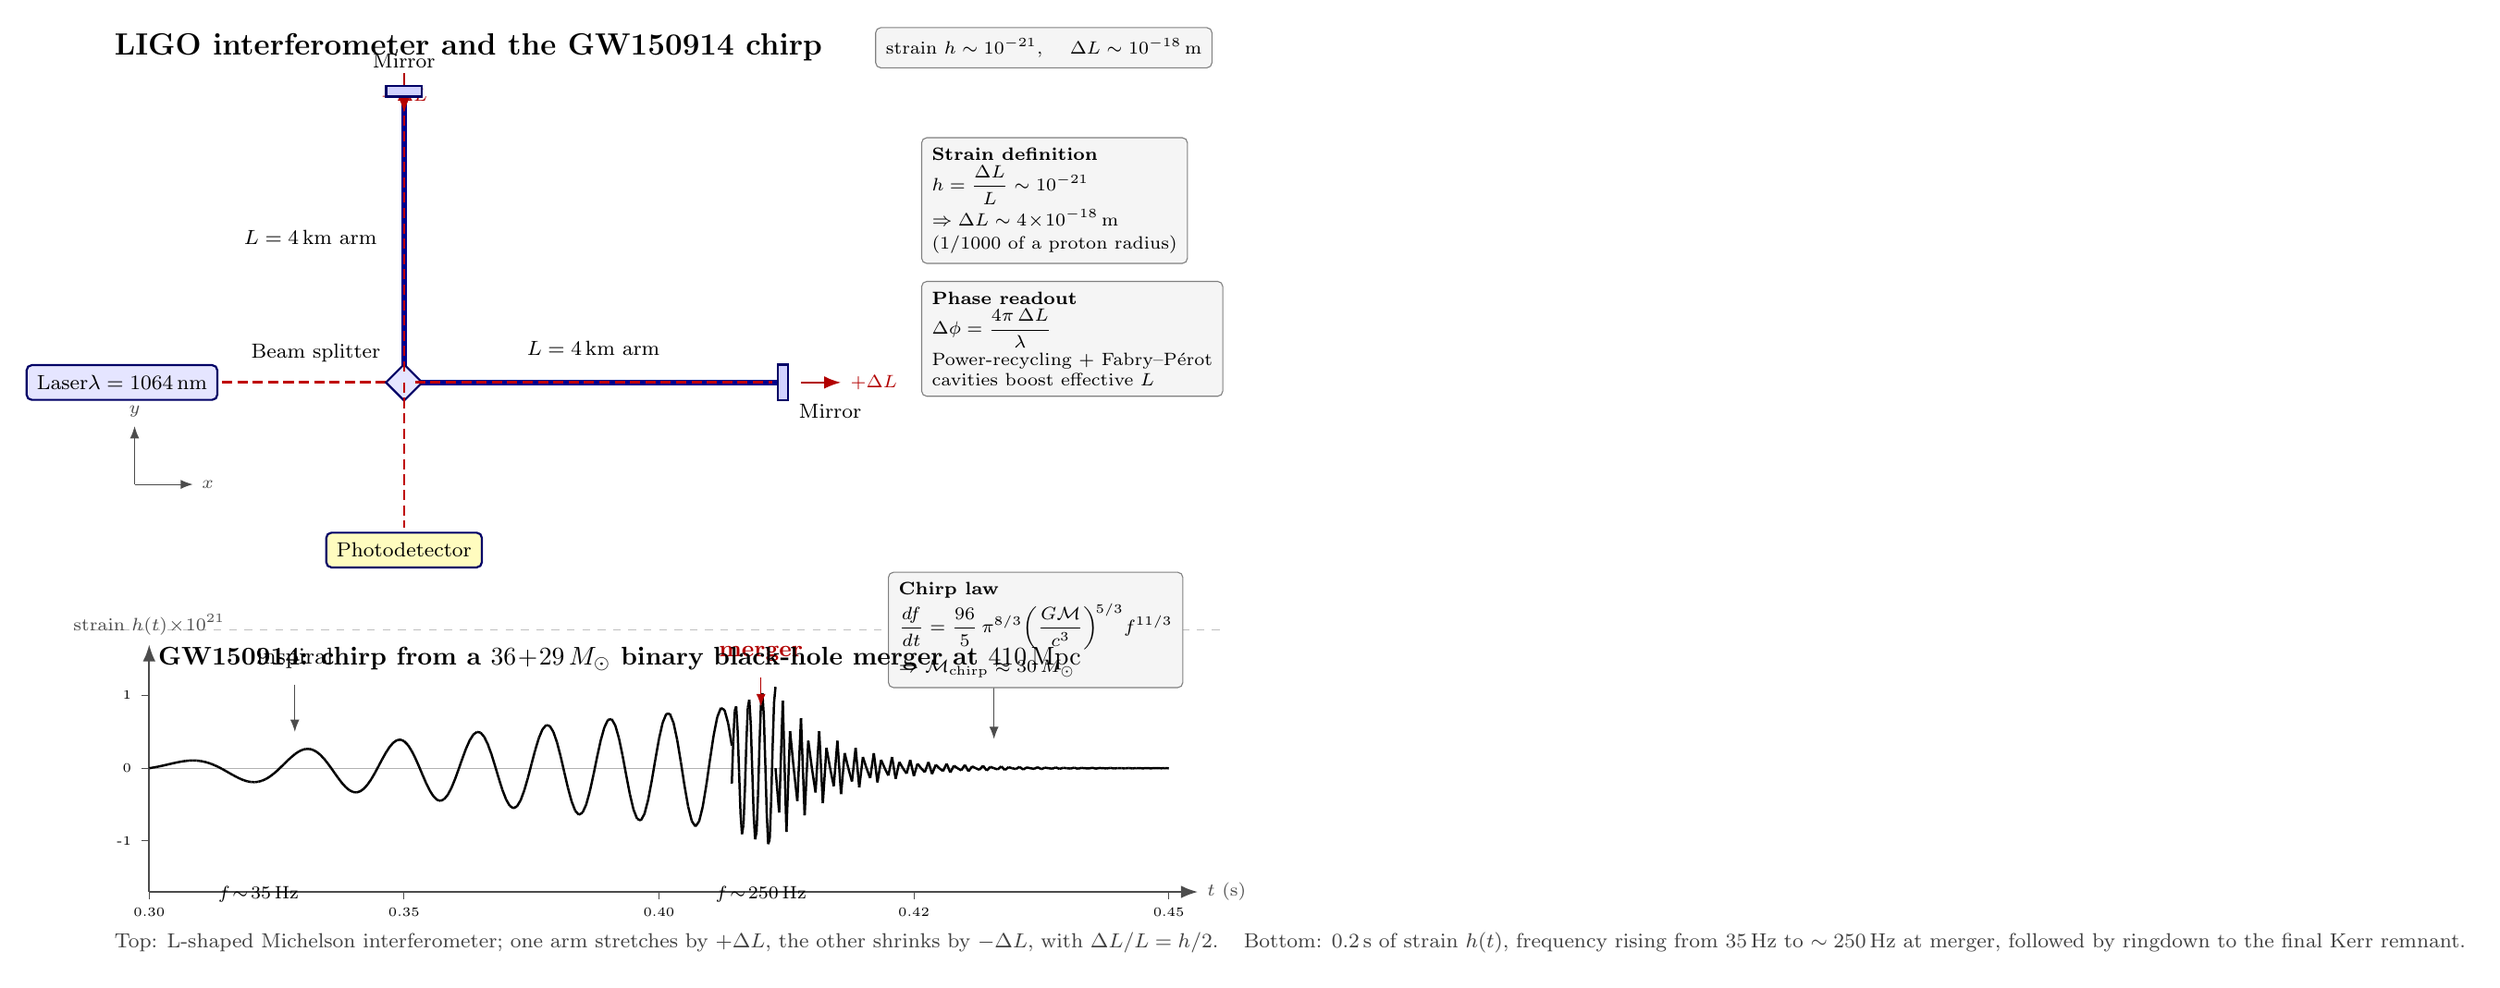
\begin{tikzpicture}[>=Latex,
  arm/.style={draw=blue!55!black, line width=2.0pt},
  laser/.style={draw=red!75!black, line width=1.0pt, dash pattern=on 4pt off 2pt},
  mirror/.style={draw=blue!40!black, fill=blue!18, thick, minimum width=14pt, minimum height=4pt, inner sep=0pt},
  splitter/.style={draw=blue!40!black, fill=blue!10, thick, minimum size=10pt, inner sep=0pt, rotate=45},
  device/.style={draw=blue!40!black, fill=blue!10, thick, rounded corners=2pt, inner sep=4pt, font=\footnotesize},
  detector/.style={draw=blue!40!black, fill=yellow!25, thick, rounded corners=2pt, inner sep=4pt, font=\footnotesize},
  lab/.style={font=\footnotesize},
  axislab/.style={font=\scriptsize, gray!60!black},
  notebox/.style={rectangle, draw=black!50, thin, rounded corners=2pt, fill=gray!8, inner sep=4pt, align=left, font=\scriptsize}]

  % ============================================================
  %  TOP: title banner
  % ============================================================
  \node[font=\large\bfseries, anchor=west] at (-7.6, 8.6)
    {LIGO interferometer and the GW150914 chirp};
  \node[notebox, anchor=east] at (7.6, 8.6)
    {strain $h \sim 10^{-21}$, \quad $\Delta L \sim 10^{-18}\,\mathrm{m}$};

  % ============================================================
  %  UPPER HALF: Michelson-style interferometer (L-shape)
  % ============================================================

  % Origin of the L: beam splitter at (-3.5, 4.0)
  \coordinate (BS)  at (-3.5, 4.0);
  \coordinate (LAS) at (-6.0, 4.0);   % laser to the left
  \coordinate (MX)  at (1.7,  4.0);   % end mirror, x-arm (right)
  \coordinate (MY)  at (-3.5, 8.0);   % end mirror, y-arm (up)
  \coordinate (PD)  at (-3.5, 2.0);   % photodetector below splitter

  % --- two arms (4 km each, schematic) ---
  \draw[arm] (BS) -- (MX);
  \draw[arm] (BS) -- (MY);

  % --- arm length labels ---
  \node[lab, above] at ($(BS)!0.5!(MX) + (0,0.25)$) {$L = 4\,\mathrm{km}$ arm};
  \node[lab, left]  at ($(BS)!0.5!(MY) + (-0.25,0)$) {$L = 4\,\mathrm{km}$ arm};

  % --- delta L stretch indication on x-arm ---
  \draw[->, red!70!black, thick]
    ($(MX) + (0.25, 0)$) -- ++(0.55, 0)
    node[right, font=\scriptsize, red!70!black] {$+\Delta L$};
  % --- delta L compression on y-arm ---
  \draw[->, red!70!black, thick]
    ($(MY) + (0, 0.25)$) -- ++(0, -0.55)
    node[above, font=\scriptsize, red!70!black] {$-\Delta L$};

  % --- laser source ---
  \node[device, anchor=east] at ($(LAS) + (-0.05, 0)$) {Laser\\$\lambda = 1064\,\mathrm{nm}$};
  \draw[laser] (LAS) -- (BS);

  % --- beam splitter ---
  \node[splitter] at (BS) {};
  \node[lab, anchor=south east] at ($(BS) + (-0.20, 0.15)$) {Beam splitter};

  % --- end mirrors ---
  \node[mirror, rotate=90] at (MX) {};
  \node[lab, right] at ($(MX) + (0.10, -0.40)$) {Mirror};
  \node[mirror] at (MY) {};
  \node[lab, above] at ($(MY) + (0, 0.20)$) {Mirror};

  % --- internal laser paths along arms (red dashed inside arms) ---
  \draw[laser] ($(BS) + (0.15, 0)$) -- ($(MX) + (-0.15, 0)$);
  \draw[laser] ($(BS) + (0, 0.15)$) -- ($(MY) + (0, -0.15)$);

  % --- photodetector below splitter ---
  \draw[laser] (BS) -- (PD);
  \node[detector, anchor=north] at ($(PD) + (0, -0.05)$) {Photodetector};

  % --- coordinate axes (small, lower left) ---
  \draw[->, gray!60!black, thin] (-7.2, 2.6) -- (-6.4, 2.6) node[axislab, right] {$x$};
  \draw[->, gray!60!black, thin] (-7.2, 2.6) -- (-7.2, 3.4) node[axislab, above] {$y$};

  % --- strain note on the right ---
  \node[notebox, anchor=west] at (3.6, 6.5) {%
    \textbf{Strain definition}\\[1pt]
    $h = \dfrac{\Delta L}{L}\sim 10^{-21}$\\[1pt]
    $\Rightarrow \Delta L \sim 4\!\times\!10^{-18}\,\mathrm{m}$\\[1pt]
    (1/1000 of a proton radius)};

  \node[notebox, anchor=west] at (3.6, 4.6) {%
    \textbf{Phase readout}\\[1pt]
    $\Delta\phi = \dfrac{4\pi\,\Delta L}{\lambda}$\\[1pt]
    Power-recycling + Fabry--P\'erot\\
    cavities boost effective $L$};

  % ============================================================
  %  Separator
  % ============================================================
  \draw[gray!50, dashed] (-7.8, 0.6) -- (7.8, 0.6);

  % ============================================================
  %  LOWER HALF: GW150914 chirp waveform
  % ============================================================

  % --- axes for the chirp plot ---
  \coordinate (W0) at (-7.0, -3.0);  % origin of waveform plot
  \draw[->, black!70, thick] (W0) -- ++(14.4, 0) node[right, font=\scriptsize] {$t$ (s)};
  \draw[->, black!70, thick] (W0) -- ++(0, 3.4) node[above, font=\scriptsize] {strain $h(t)\!\times\!10^{21}$};

  % --- horizontal zero-line for clarity ---
  \draw[black!30, thin] ($(W0) + (0, 1.7)$) -- ++(14.0, 0);

  % --- time axis ticks ---
  \foreach \x/\lab in {0.0/0.30, 3.5/0.35, 7.0/0.40, 10.5/0.42, 14.0/0.45} {
    \draw[black!70, thin] ($(W0) + (\x, 0)$) -- ++(0, -0.10);
    \node[font=\tiny, below] at ($(W0) + (\x, -0.10)$) {\lab};
  }

  % --- strain ticks (left side) ---
  \foreach \y/\lab in {0.7/-1, 1.7/0, 2.7/1} {
    \draw[black!70, thin] ($(W0) + (0, \y)$) -- ++(-0.10, 0);
    \node[font=\tiny, anchor=east] at ($(W0) + (-0.12, \y)$) {\lab};
  }

  % --- chirp signal: amplitude grows, frequency grows, then peak, then ringdown ---
  % We build the waveform as a piecewise smooth curve:
  %   t in [0,8]  : inspiral, A grows ~ t, omega grows roughly ~ (1-t/9)^{-3/8}
  %   t in [8,9]  : merger peak
  %   t in [9,12] : ringdown (decaying sinusoid)
  % Implemented as a dense \foreach plotting black dots/lines.

  % We sample with many small \draw segments to avoid TikZ dimension overflow.
  % The waveform is centred on y = 1.7 inside the plot frame whose origin is W0.

  % --- inspiral: 0 <= s <= 8 (s = local time)
  % amplitude: A(s) = 0.05 + 0.10*s  (max ~0.85 near s=8)
  % frequency factor: f(s) grows linearly so phase ~ 0.45*s + 0.06*s^2 (cycles)
  % Phase wrapped mod 360 to avoid pgfmath dimension overflow.
  \foreach \i in {0,...,159} {
    \pgfmathsetmacro{\sA}{\i*0.05}
    \pgfmathsetmacro{\sB}{(\i+1)*0.05}
    \pgfmathsetmacro{\ampA}{0.05 + 0.10*\sA}
    \pgfmathsetmacro{\ampB}{0.05 + 0.10*\sB}
    \pgfmathsetmacro{\rawA}{0.45*\sA + 0.06*\sA*\sA}
    \pgfmathsetmacro{\rawB}{0.45*\sB + 0.06*\sB*\sB}
    \pgfmathsetmacro{\fracA}{\rawA - int(\rawA)}
    \pgfmathsetmacro{\fracB}{\rawB - int(\rawB)}
    \pgfmathsetmacro{\phA}{360*\fracA}
    \pgfmathsetmacro{\phB}{360*\fracB}
    \pgfmathsetmacro{\yA}{1.7 + \ampA*sin(\phA)}
    \pgfmathsetmacro{\yB}{1.7 + \ampB*sin(\phB)}
    \draw[black, line width=0.9pt]
      ($(W0) + (\sA, \yA)$) -- ($(W0) + (\sB, \yB)$);
  }

  % --- merger ramp: 8 <= s <= 8.6, rapid rise to peak
  \foreach \i in {0,...,29} {
    \pgfmathsetmacro{\sA}{8.0 + \i*0.02}
    \pgfmathsetmacro{\sB}{8.0 + (\i+1)*0.02}
    \pgfmathsetmacro{\dA}{\sA-8.0}
    \pgfmathsetmacro{\dB}{\sB-8.0}
    \pgfmathsetmacro{\ampA}{0.85 + 0.45*\dA}
    \pgfmathsetmacro{\ampB}{0.85 + 0.45*\dB}
    \pgfmathsetmacro{\rawA}{5.5*\dA + 4.96}
    \pgfmathsetmacro{\rawB}{5.5*\dB + 4.96}
    \pgfmathsetmacro{\fracA}{\rawA - int(\rawA)}
    \pgfmathsetmacro{\fracB}{\rawB - int(\rawB)}
    \pgfmathsetmacro{\phA}{360*\fracA}
    \pgfmathsetmacro{\phB}{360*\fracB}
    \pgfmathsetmacro{\yA}{1.7 + \ampA*sin(\phA)}
    \pgfmathsetmacro{\yB}{1.7 + \ampB*sin(\phB)}
    \draw[black, line width=0.9pt]
      ($(W0) + (\sA, \yA)$) -- ($(W0) + (\sB, \yB)$);
  }

  % --- ringdown: 8.6 <= s <= 14.0, decaying sinusoid
  \foreach \i in {0,...,107} {
    \pgfmathsetmacro{\sA}{8.6 + \i*0.05}
    \pgfmathsetmacro{\sB}{8.6 + (\i+1)*0.05}
    \pgfmathsetmacro{\dA}{\sA-8.6}
    \pgfmathsetmacro{\dB}{\sB-8.6}
    \pgfmathsetmacro{\envA}{1.10*exp(-1.2*\dA)}
    \pgfmathsetmacro{\envB}{1.10*exp(-1.2*\dB)}
    \pgfmathsetmacro{\rawA}{8.0*\dA + 5.5}
    \pgfmathsetmacro{\rawB}{8.0*\dB + 5.5}
    \pgfmathsetmacro{\fracA}{\rawA - int(\rawA)}
    \pgfmathsetmacro{\fracB}{\rawB - int(\rawB)}
    \pgfmathsetmacro{\phA}{360*\fracA}
    \pgfmathsetmacro{\phB}{360*\fracB}
    \pgfmathsetmacro{\yA}{1.7 + \envA*sin(\phA)}
    \pgfmathsetmacro{\yB}{1.7 + \envB*sin(\phB)}
    \draw[black, line width=0.9pt]
      ($(W0) + (\sA, \yA)$) -- ($(W0) + (\sB, \yB)$);
  }

  % --- annotations on waveform ---
  \node[font=\small, anchor=south] at ($(W0) + (2.0, 2.95)$) {inspiral};
  \draw[black!70, thin, ->] ($(W0) + (2.0, 2.85)$) -- ($(W0) + (2.0, 2.20)$);

  \node[font=\small\bfseries, anchor=south, red!70!black] at ($(W0) + (8.4, 3.05)$) {merger};
  \draw[red!70!black, thin, ->] ($(W0) + (8.4, 2.95)$) -- ($(W0) + (8.4, 2.55)$);

  \node[font=\small, anchor=south] at ($(W0) + (11.6, 2.95)$) {ringdown};
  \draw[black!70, thin, ->] ($(W0) + (11.6, 2.85)$) -- ($(W0) + (11.6, 2.10)$);

  % --- frequency annotations ---
  \node[font=\scriptsize, anchor=north] at ($(W0) + (1.5, 0.20)$) {$f \!\sim\! 35\,\mathrm{Hz}$};
  \node[font=\scriptsize, anchor=north] at ($(W0) + (8.4, 0.20)$) {$f \!\sim\! 250\,\mathrm{Hz}$};

  % --- chirp formula box ---
  \node[notebox, anchor=south east] at ($(W0) + (14.2, 2.8)$) {%
    \textbf{Chirp law}\\[1pt]
    $\dfrac{df}{dt} = \dfrac{96}{5}\,\pi^{8/3}
       \!\left(\dfrac{G\mathcal{M}}{c^3}\right)^{\!5/3}\! f^{11/3}$\\[3pt]
    $\Rightarrow \mathcal{M}_{\rm chirp} \approx 30\,M_\odot$};

  % --- title for lower half ---
  \node[font=\bfseries, anchor=west] at (-7.0, 0.20)
    {GW150914: chirp from a $36\!+\!29\,M_\odot$ binary black-hole merger at $410\,\mathrm{Mpc}$};

  % ============================================================
  %  Bottom legend
  % ============================================================
  \node[font=\footnotesize, anchor=west, text=black!75]
    at (-7.6, -3.7)
    {Top: L-shaped Michelson interferometer; one arm stretches by $+\Delta L$, the other shrinks
     by $-\Delta L$, with $\Delta L/L = h/2$. \;
     Bottom: 0.2\,s of strain $h(t)$, frequency rising from $35\,\mathrm{Hz}$ to $\sim 250\,\mathrm{Hz}$
     at merger, followed by ringdown to the final Kerr remnant.};

\end{tikzpicture}
\end{document}
